\documentclass[12pt,a4paper]{article}

% ---------------------------------------------------------------
% PACKAGES
% ---------------------------------------------------------------
\usepackage{amsmath}
\usepackage{amssymb}
\usepackage{geometry}
\geometry{margin=2.5cm}
\usepackage{booktabs}
\usepackage{xcolor}
\usepackage{hyperref}
\usepackage{listings}
\usepackage{pgfplots}
\pgfplotsset{compat=1.18}
\usepackage[most,breakable]{tcolorbox}
\tcbuselibrary{skins, breakable}
\usepackage{enumitem}
\usepackage{fancyhdr}
\usepackage{tikz}
\usepackage{array}

% ---------------------------------------------------------------
% TCOLORBOX ENVIRONMENTS
% ---------------------------------------------------------------
\newtcolorbox{curiositybox}[1]{colback=yellow!10, colframe=orange!80!black, fonttitle=\bfseries, title=#1, breakable}
\newtcolorbox{infobox}[1]{colback=blue!5, colframe=blue!60!black, fonttitle=\bfseries, title=#1, breakable}
\newtcolorbox{mistakebox}[1]{colback=red!5, colframe=red!60!black, fonttitle=\bfseries, title=#1, breakable}
\newtcolorbox{learnbox}[1]{colback=green!5, colframe=green!60!black, fonttitle=\bfseries, title=#1, breakable}

% ---------------------------------------------------------------
% LISTINGS SETUP
% ---------------------------------------------------------------
\lstset{language=Python, basicstyle=\ttfamily\small, keywordstyle=\color{blue},
        commentstyle=\color{gray}, stringstyle=\color{red},
        showstringspaces=false, breaklines=true, frame=single}

% ---------------------------------------------------------------
% FANCYHDR
% ---------------------------------------------------------------
\pagestyle{fancy}
\fancyhf{}
\lhead{Topic 13: Taylor Series}
\rhead{Unit II --- Complex Variables}
\cfoot{\thepage}

% ---------------------------------------------------------------
% TITLE
% ---------------------------------------------------------------
\title{\textbf{Topic 13: Power Series Expansions --- Taylor's Series}\\
\large Unit II: Complex Variable: Integration\\
Complex Variables and Special Functions\\
JNTUA College of Engineering (Autonomous)}
\author{B.Tech Engineering Students}
\date{}

% ---------------------------------------------------------------
\begin{document}
\maketitle
\tableofcontents
\newpage

% ===============================================================
% OPENING HOOK
% ===============================================================
\begin{curiositybox}{Hook}
In real calculus, a Taylor series is a useful approximation. In complex analysis, something remarkable happens: if a function is analytic, it is not just approximately equal to a power series near a point --- it actually \emph{becomes} that power series. This is one of the most striking differences between real and complex analysis: analyticity forces the function to be \emph{exactly} representable as a convergent power series in every disk that avoids singularities.
\end{curiositybox}

\bigskip

% ===============================================================
% SECTION 1: From Real Taylor Series to Complex Taylor Series
% ===============================================================
\section{From Real Taylor Series to Complex Taylor Series}

In real analysis, the Taylor series of a smooth function $f(x)$ about a point $x_0$ is
\[
  f(x) = \sum_{n=0}^{\infty} \frac{f^{(n)}(x_0)}{n!}(x - x_0)^n,
\]
valid in some interval $(x_0 - R,\, x_0 + R)$. This requires that $f$ be \emph{infinitely differentiable} --- a condition that many real functions fail to satisfy globally, even if they look smooth locally.

Complex analysis changes the story fundamentally. The single hypothesis that $f(z)$ is \emph{analytic} (holomorphic) in a domain $D$ already guarantees that $f$ possesses derivatives of \emph{all orders} in $D$. As a consequence, any analytic function \emph{automatically} has a Taylor expansion that converges to it exactly, not merely as an approximation.

\begin{center}
\begin{tabular}{lll}
\toprule
\textbf{Property} & \textbf{Real Taylor} & \textbf{Complex Taylor} \\
\midrule
Hypothesis & $C^\infty$ at $x_0$ & Analytic in a disk about $z_0$ \\
Convergence & Interval $(x_0-R,x_0+R)$ & Open disk $|z-z_0|<R$ \\
Equality & Series may not equal $f$ & Series equals $f$ exactly inside disk \\
Radius limit & Hard to determine & Nearest singularity of $f$ \\
\bottomrule
\end{tabular}
\end{center}

\begin{learnbox}{Key Takeaway}
In complex analysis, analytic $\Rightarrow$ all derivatives exist $\Rightarrow$ Taylor series converges to the function exactly in every disk free of singularities.
\end{learnbox}

% ===============================================================
% SECTION 2: Statement of Taylor's Theorem
% ===============================================================
\section{Statement of Taylor Series for Analytic Functions}

\begin{infobox}{Taylor's Theorem for Analytic Functions}
Let $f(z)$ be analytic everywhere inside a disk $|z - z_0| < R$ (where $R > 0$). Then $f(z)$ can be represented inside that disk by the \textbf{Taylor series}:
\[
  f(z) = \sum_{n=0}^{\infty} \frac{f^{(n)}(z_0)}{n!}(z - z_0)^n
       = f(z_0) + f'(z_0)(z-z_0) + \frac{f''(z_0)}{2!}(z-z_0)^2 + \cdots
\]
The coefficients are given by the \textbf{Cauchy Integral Formula for derivatives}:
\[
  f^{(n)}(z_0) = \frac{n!}{2\pi i} \oint_{C} \frac{f(z)}{(z-z_0)^{n+1}}\,dz,
\]
so equivalently:
\[
  a_n = \frac{f^{(n)}(z_0)}{n!} = \frac{1}{2\pi i} \oint_{C} \frac{f(z)}{(z-z_0)^{n+1}}\,dz.
\]
The series converges absolutely and uniformly for $|z - z_0| < R$.
\end{infobox}

\paragraph{Center $z_0$ and Radius of Convergence $R$.}
The point $z_0$ is called the \emph{center} of the expansion. The radius of convergence $R$ is the distance from $z_0$ to the nearest singularity of $f$. Inside the disk $|z - z_0| < R$ the series converges to $f(z)$; outside the disk ($|z - z_0| > R$) the series diverges. On the circle $|z - z_0| = R$ convergence must be tested separately.

\begin{learnbox}{Radius of Convergence}
$R = $ distance from $z_0$ to the nearest singularity of $f$. There is \emph{always} a singularity on the circle $|z-z_0|=R$ (otherwise the disk could be enlarged).
\end{learnbox}

% ===============================================================
% SECTION 3: Maclaurin Series as Special Case
% ===============================================================
\section{Maclaurin Series as Special Case}

When the center is chosen to be $z_0 = 0$, the Taylor series reduces to the \textbf{Maclaurin series}:

\begin{infobox}{Maclaurin Series ($z_0 = 0$)}
\[
  f(z) = \sum_{n=0}^{\infty} \frac{f^{(n)}(0)}{n!}\,z^n
       = f(0) + f'(0)\,z + \frac{f''(0)}{2!}\,z^2 + \frac{f'''(0)}{3!}\,z^3 + \cdots
\]
This is valid in the largest disk $|z| < R$ centred at the origin in which $f$ is analytic.
\end{infobox}

All the classical standard expansions ($e^z$, $\sin z$, $\cos z$, $1/(1-z)$, $\log(1+z)$) are Maclaurin series. The Maclaurin series is simply the ``default'' expansion used when there is no reason to choose a different center.

\begin{learnbox}{Maclaurin = Taylor at Origin}
Maclaurin series is the Taylor series centred at $z_0 = 0$. It is the most commonly tabulated form of standard expansions.
\end{learnbox}

% ===============================================================
% SECTION 4: Radius of Convergence and Analytic Region
% ===============================================================
\section{Radius of Convergence and Analytic Region}

\begin{infobox}{Determining the Radius of Convergence}
For a Taylor series $\displaystyle\sum_{n=0}^{\infty} a_n (z-z_0)^n$, the radius of convergence $R$ can be computed by:
\begin{itemize}[noitemsep]
  \item \textbf{Ratio test:} $R = \displaystyle\lim_{n\to\infty}\left|\frac{a_n}{a_{n+1}}\right|$ (when the limit exists).
  \item \textbf{Root test (Hadamard formula):} $\dfrac{1}{R} = \displaystyle\limsup_{n\to\infty} |a_n|^{1/n}$.
  \item \textbf{Geometric rule:} $R = $ distance from $z_0$ to the nearest singularity of $f$ in $\mathbb{C}$.
\end{itemize}
Inside $|z - z_0| < R$: series converges absolutely.\\
Outside $|z - z_0| > R$: series diverges.
\end{infobox}

\subsection*{Diagram: Convergence Disk and Nearest Singularity}

\begin{center}
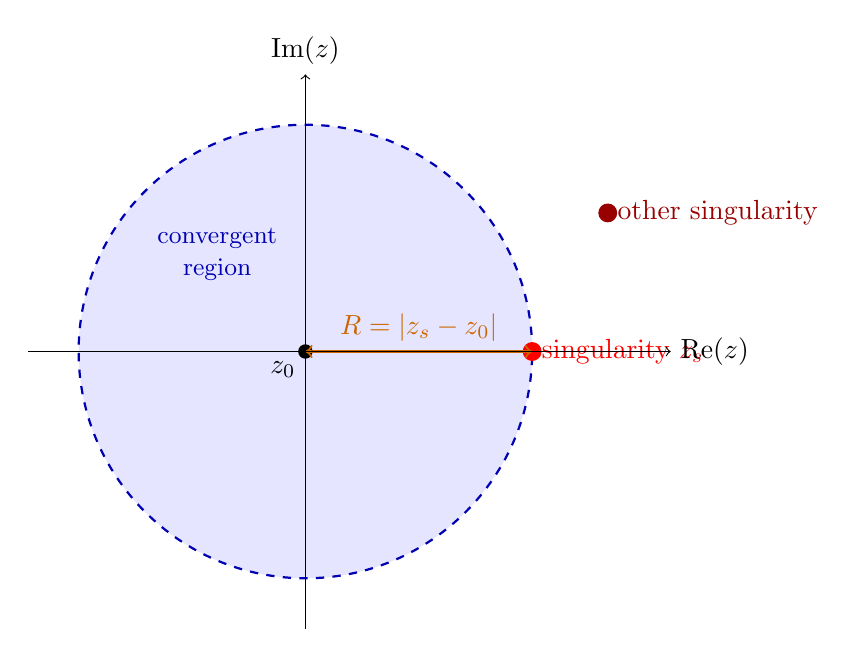
\begin{tikzpicture}[scale=1.6]
  % Shaded convergence disk
  \fill[blue!10] (0,0) circle (1.8cm);
  % Boundary circle
  \draw[blue!70!black, thick, dashed] (0,0) circle (1.8cm);
  % Center z0
  \filldraw[black] (0,0) circle (1.5pt) node[below left] {$z_0$};
  % Nearest singularity on boundary
  \filldraw[red] (1.8,0) circle (2pt) node[right] {singularity $z_s$};
  % Another singularity outside the disk
  \filldraw[red!60!black] (2.4,1.1) circle (2pt) node[right] {other singularity};
  % Radius arrow
  \draw[<->, thick, orange!80!black] (0,0) -- node[above, sloped] {$R = |z_s - z_0|$} (1.8,0);
  % Axes
  \draw[->] (-2.2,0) -- (2.9,0) node[right] {$\operatorname{Re}(z)$};
  \draw[->] (0,-2.2) -- (0,2.2) node[above] {$\operatorname{Im}(z)$};
  % Label convergent region
  \node[blue!70!black] at (-0.7,0.9) {\small convergent};
  \node[blue!70!black] at (-0.7,0.65) {\small region};
\end{tikzpicture}
\end{center}

The series converges in the entire shaded disk $|z - z_0| < R$ and diverges outside. The radius $R$ equals the distance to the \emph{nearest} singularity; more distant singularities do not further restrict the disk.

\begin{learnbox}{Singularity Governs Radius}
To find $R$ quickly: locate all singularities of $f$ in $\mathbb{C}$, and $R$ equals the distance from $z_0$ to the closest one. If $f$ is entire (no singularities), then $R = \infty$.
\end{learnbox}

% ===============================================================
% SECTION 5: Standard Expansions
% ===============================================================
\section{Standard Expansions}

\begin{infobox}{Standard Maclaurin Series}
The following are valid for all $z \in \mathbb{C}$ unless otherwise stated.

\medskip
\begin{tabular}{ll}
\toprule
\textbf{Function} & \textbf{Maclaurin Series} \\
\midrule
$e^z$ & $\displaystyle\sum_{n=0}^{\infty}\dfrac{z^n}{n!} = 1 + z + \dfrac{z^2}{2!} + \dfrac{z^3}{3!} + \cdots$, \quad $|z| < \infty$ \\[8pt]
$\sin z$ & $\displaystyle\sum_{n=0}^{\infty}\dfrac{(-1)^n z^{2n+1}}{(2n+1)!} = z - \dfrac{z^3}{3!} + \dfrac{z^5}{5!} - \cdots$, \quad $|z| < \infty$ \\[8pt]
$\cos z$ & $\displaystyle\sum_{n=0}^{\infty}\dfrac{(-1)^n z^{2n}}{(2n)!} = 1 - \dfrac{z^2}{2!} + \dfrac{z^4}{4!} - \cdots$, \quad $|z| < \infty$ \\[8pt]
$\dfrac{1}{1-z}$ & $\displaystyle\sum_{n=0}^{\infty} z^n = 1 + z + z^2 + z^3 + \cdots$, \quad $|z| < 1$ \\[8pt]
$\log(1+z)$ & $\displaystyle\sum_{n=1}^{\infty}\dfrac{(-1)^{n+1}z^n}{n} = z - \dfrac{z^2}{2} + \dfrac{z^3}{3} - \cdots$, \quad $|z| < 1$ \\[8pt]
$(1+z)^m$ & $\displaystyle\sum_{n=0}^{\infty}\binom{m}{n}z^n$, \quad $|z| < 1$ (generalized binomial) \\
\bottomrule
\end{tabular}
\end{infobox}

\paragraph{Why do $e^z$, $\sin z$, $\cos z$ converge everywhere?} These functions are entire (no singularities in $\mathbb{C}$), so $R = \infty$ and the series converge for every $z \in \mathbb{C}$. In contrast, $1/(1-z)$ has a singularity at $z = 1$, so its Maclaurin series only converges for $|z| < 1$.

\begin{learnbox}{Entire vs.\ Singular Functions}
Entire functions ($e^z$, $\sin z$, $\cos z$, polynomials) have $R=\infty$. Functions with poles or branch points have $R = $ distance to the nearest singularity.
\end{learnbox}

% ===============================================================
% SECTION 6: Worked Examples
% ===============================================================
\section{Worked Examples}

% ------- Example 1 -------
\subsection*{Example 1: Maclaurin Series of $e^z$}

\textbf{Find the Taylor series of $f(z) = e^z$ about $z_0 = 0$.}

\medskip
We compute successive derivatives: $f^{(n)}(z) = e^z$ for all $n \geq 0$, so $f^{(n)}(0) = e^0 = 1$.

Substituting into the Taylor formula:
\[
  e^z = \sum_{n=0}^{\infty} \frac{1}{n!}\,z^n = 1 + z + \frac{z^2}{2!} + \frac{z^3}{3!} + \frac{z^4}{4!} + \cdots
\]
Since $e^z$ has no singularities, $R = \infty$: the series converges for all $z \in \mathbb{C}$.

\begin{learnbox}{Example 1 Result}
$e^z = \displaystyle\sum_{n=0}^{\infty}\dfrac{z^n}{n!}$, convergent for all $z \in \mathbb{C}$ ($R = \infty$).
\end{learnbox}

% ------- Example 2 -------
\subsection*{Example 2: Maclaurin Series of $\sin z$}

\textbf{Find the Taylor series of $f(z) = \sin z$ about $z_0 = 0$.}

\medskip
Derivatives cycle with period 4:
\[
  f(z) = \sin z,\quad f'(z) = \cos z,\quad f''(z) = -\sin z,\quad f'''(z) = -\cos z,\quad f^{(4)}(z) = \sin z,\;\ldots
\]
At $z = 0$:
\[
  f(0)=0,\quad f'(0)=1,\quad f''(0)=0,\quad f'''(0)=-1,\quad f^{(4)}(0)=0,\quad f^{(5)}(0)=1,\;\ldots
\]
Only odd-order derivatives are nonzero, so:
\[
  \sin z = z - \frac{z^3}{3!} + \frac{z^5}{5!} - \frac{z^7}{7!} + \cdots = \sum_{n=0}^{\infty} \frac{(-1)^n\,z^{2n+1}}{(2n+1)!}
\]
Again $R = \infty$ since $\sin z$ is entire.

\begin{learnbox}{Example 2 Result}
$\sin z = \displaystyle\sum_{n=0}^{\infty}\dfrac{(-1)^n z^{2n+1}}{(2n+1)!}$, valid for all $z \in \mathbb{C}$.
\end{learnbox}

% ------- Example 3 -------
\subsection*{Example 3: Taylor Series of $\dfrac{1}{1-z}$ about $z_0 = 0$}

\textbf{Find the Maclaurin series of $f(z) = \dfrac{1}{1-z}$ and state its radius of convergence.}

\medskip
Derivatives: $f^{(n)}(z) = \dfrac{n!}{(1-z)^{n+1}}$, so $f^{(n)}(0) = n!$.

Therefore:
\[
  a_n = \frac{f^{(n)}(0)}{n!} = \frac{n!}{n!} = 1, \quad \text{for all } n \geq 0.
\]
\[
  \frac{1}{1-z} = \sum_{n=0}^{\infty} z^n = 1 + z + z^2 + z^3 + \cdots
\]
The singularity is at $z = 1$, so $R = |1 - 0| = 1$. The series converges for $|z| < 1$.

\begin{learnbox}{Example 3 Result}
$\dfrac{1}{1-z} = \displaystyle\sum_{n=0}^{\infty} z^n$, valid for $|z| < 1$. This is the complex geometric series.
\end{learnbox}

% ------- Example 4 -------
\subsection*{Example 4: Taylor Series of $\dfrac{1}{1+z^2}$ about $z_0 = 0$}

\textbf{Expand $f(z) = \dfrac{1}{1+z^2}$ as a Maclaurin series and find $R$.}

\medskip
Replace $z$ with $-z^2$ in the geometric series $\dfrac{1}{1-w} = \sum_{n=0}^{\infty} w^n$ (valid $|w|<1$):
\[
  \frac{1}{1+z^2} = \frac{1}{1-(-z^2)} = \sum_{n=0}^{\infty} (-z^2)^n = \sum_{n=0}^{\infty} (-1)^n z^{2n}
  = 1 - z^2 + z^4 - z^6 + \cdots
\]
The singularities of $f$ are at $z^2 = -1$, i.e.\ $z = \pm i$. The distance from $z_0 = 0$ to $z = i$ is $|i - 0| = 1$, so $R = 1$.

The series converges for $|z| < 1$.

\begin{learnbox}{Example 4 Result}
$\dfrac{1}{1+z^2} = \displaystyle\sum_{n=0}^{\infty}(-1)^n z^{2n}$, valid for $|z|<1$. Singularities at $z=\pm i$ set $R=1$.
\end{learnbox}

% ------- Example 5 -------
\subsection*{Example 5: Expansion about a Nonzero Center --- $e^z$ about $z_0 = 1$}

\textbf{Expand $f(z) = e^z$ in a Taylor series about $z_0 = 1$.}

\medskip
All derivatives satisfy $f^{(n)}(z) = e^z$, so $f^{(n)}(z_0) = f^{(n)}(1) = e^1 = e$.

\[
  e^z = \sum_{n=0}^{\infty} \frac{e}{n!}(z-1)^n = e\sum_{n=0}^{\infty}\frac{(z-1)^n}{n!}
      = e\left[1 + (z-1) + \frac{(z-1)^2}{2!} + \frac{(z-1)^3}{3!} + \cdots\right]
\]
Since $e^z$ is entire, $R = \infty$.

\textit{Verification:} Let $z = 1 + w$. Then $e^z = e^{1+w} = e \cdot e^w = e\sum_{n=0}^{\infty}\dfrac{w^n}{n!}$, which matches. \checkmark

\begin{learnbox}{Example 5 Result}
$e^z = e\displaystyle\sum_{n=0}^{\infty}\dfrac{(z-1)^n}{n!}$ about $z_0=1$, valid for all $z\in\mathbb{C}$.
\end{learnbox}

% ------- Example 6 -------
\subsection*{Example 6: Taylor Series of $\cos z$ about $z_0 = 0$}

\textbf{Derive the Maclaurin series for $f(z) = \cos z$.}

\medskip
Even-numbered derivatives survive at $z=0$:
\[
  f^{(0)}(0)=1,\quad f^{(2)}(0)=-1,\quad f^{(4)}(0)=1,\quad f^{(2k)}(0)=(-1)^k.
\]
All odd derivatives vanish at $z=0$. Therefore:
\[
  \cos z = \sum_{n=0}^{\infty} \frac{(-1)^n\,z^{2n}}{(2n)!}
         = 1 - \frac{z^2}{2!} + \frac{z^4}{4!} - \frac{z^6}{6!} + \cdots
\]
Valid for all $z \in \mathbb{C}$ since $\cos z$ is entire ($R = \infty$).

\begin{learnbox}{Example 6 Result}
$\cos z = \displaystyle\sum_{n=0}^{\infty}\dfrac{(-1)^n z^{2n}}{(2n)!}$, valid for all $z \in \mathbb{C}$.
\end{learnbox}

% ------- Example 7 -------
\subsection*{Example 7: Deriving Coefficients via the Cauchy Integral Formula}

\textbf{Use the Cauchy Integral Formula to find the coefficient $a_2$ in the Taylor expansion of $f(z) = \dfrac{z}{(z+1)(z+3)}$ about $z_0 = 0$.}

\medskip
The formula gives:
\[
  a_2 = \frac{f^{(2)}(0)}{2!} = \frac{1}{2\pi i}\oint_{C}\frac{f(z)}{z^{3}}\,dz
      = \frac{1}{2\pi i}\oint_{C}\frac{1}{z^2(z+1)(z+3)}\,dz,
\]
where $C$ is any circle centred at $0$ with radius $r < 1$ (so that $z=-1$ and $z=-3$ lie outside $C$).

Inside $C$ there is only the singularity at $z=0$ (a double pole). Using partial fractions on $\dfrac{1}{(z+1)(z+3)} = \dfrac{1/2}{z+1} - \dfrac{1/2}{z+3}$, we expand about $z=0$:
\[
  \frac{1}{z+1} = 1 - z + z^2 - \cdots,\qquad \frac{1}{z+3} = \frac{1}{3}\left(1 - \frac{z}{3} + \frac{z^2}{9}-\cdots\right).
\]
\[
  \frac{1}{(z+1)(z+3)} = \frac{1}{2}\!\left(1-z+z^2-\cdots\right) - \frac{1}{6}\!\left(1-\tfrac{z}{3}+\tfrac{z^2}{9}-\cdots\right)
  = \frac{1}{3} - \frac{4z}{9} + \frac{13z^2}{27} - \cdots
\]
Multiplying by $\dfrac{1}{z^2}$, the residue at $z=0$ (coefficient of $1/z$) is $-4/9$. Thus by the Residue Theorem:
\[
  a_2 = \frac{1}{2\pi i}\cdot 2\pi i \cdot\left(-\frac{4}{9}\right) = -\frac{4}{9}.
\]

\begin{learnbox}{Example 7 Result}
The Cauchy Integral Formula systematically computes Taylor coefficients via contour integration: $a_n = \text{residue of } f(z)/(z-z_0)^{n+1}$ at $z_0$.
\end{learnbox}

% ------- Example 8 -------
\subsection*{Example 8: Taylor Series of $\dfrac{1}{z}$ about $z_0 = 2$}

\textbf{Expand $f(z) = \dfrac{1}{z}$ in a Taylor series about $z_0 = 2$.}

\medskip
Write $z = 2 + (z-2)$, so:
\[
  \frac{1}{z} = \frac{1}{2+(z-2)} = \frac{1}{2}\cdot\frac{1}{1+\tfrac{z-2}{2}}
              = \frac{1}{2}\cdot\frac{1}{1-\left(-\tfrac{z-2}{2}\right)}.
\]
Apply the geometric series $\dfrac{1}{1-w} = \sum_{n=0}^{\infty} w^n$ with $w = -\dfrac{z-2}{2}$, valid for $|w|<1$, i.e.\ $|z-2|<2$:
\[
  \frac{1}{z} = \frac{1}{2}\sum_{n=0}^{\infty}\left(-\frac{z-2}{2}\right)^n
              = \frac{1}{2}\sum_{n=0}^{\infty}\frac{(-1)^n(z-2)^n}{2^n}
              = \sum_{n=0}^{\infty}\frac{(-1)^n(z-2)^n}{2^{n+1}}.
\]
The singularity of $f$ is at $z=0$; the distance from $z_0=2$ to $z=0$ is $2$, so $R = 2$. \checkmark

\begin{learnbox}{Example 8 Result}
$\dfrac{1}{z} = \displaystyle\sum_{n=0}^{\infty}\dfrac{(-1)^n(z-2)^n}{2^{n+1}}$, valid for $|z-2|<2$. Center $z_0=2$, $R=2$.
\end{learnbox}

% ===============================================================
% SECTION 7: Radius-of-Convergence Visual (MANDATORY UPGRADE)
% ===============================================================
\section{Radius-of-Convergence Visual}

This section provides a detailed diagram illustrating how the center $z_0$, the nearest singularity, and the convergence disk relate.

\begin{center}
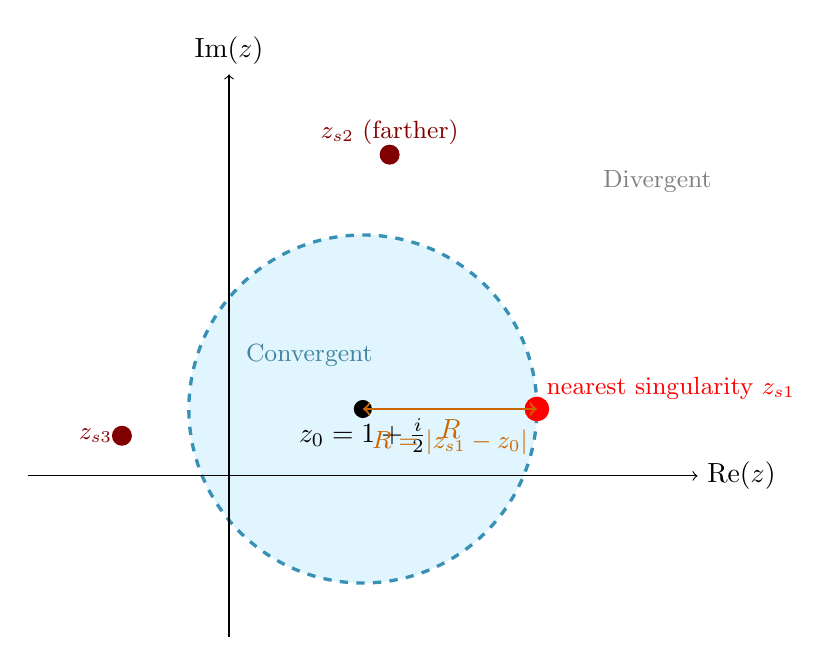
\begin{tikzpicture}[scale=1.7]
  % Convergence disk
  \fill[cyan!12] (1,0.5) circle (1.3cm);
  \draw[cyan!70!black, very thick, dashed] (1,0.5) circle (1.3cm);
  % Center
  \filldraw[black] (1,0.5) circle (1.8pt) node[below] {$z_0 = 1 + \tfrac{i}{2}$};
  % Nearest singularity
  \filldraw[red] (2.3,0.5) circle (2.5pt) node[above right] {\small nearest singularity $z_{s1}$};
  % Other singularity (farther)
  \filldraw[red!50!black] (1.2,2.4) circle (2pt) node[above] {\small $z_{s2}$ (farther)};
  % Another singularity outside
  \filldraw[red!50!black] (-0.8,0.3) circle (2pt) node[left] {\small $z_{s3}$};
  % Radius arrow
  \draw[<->, orange!80!black, thick] (1,0.5) -- node[below] {$R$} (2.3,0.5);
  % Note for R
  \node[orange!80!black, font=\small] at (1.65,0.25) {$R = |z_{s1}-z_0|$};
  % Axes
  \draw[->] (-1.5,0) -- (3.5,0) node[right] {$\operatorname{Re}(z)$};
  \draw[->] (0,-1.2) -- (0,3.0) node[above] {$\operatorname{Im}(z)$};
  % Labels inside disk
  \node[cyan!60!black, font=\small] at (0.6,0.9) {Convergent};
  % Divergent outside
  \node[gray, font=\small] at (3.2,2.2) {Divergent};
\end{tikzpicture}
\end{center}

\noindent
\textbf{Reading the diagram:}
\begin{itemize}[noitemsep]
  \item The expansion center $z_0$ is the center of the shaded disk.
  \item $z_{s1}$ is the nearest singularity, determining $R = |z_{s1} - z_0|$.
  \item $z_{s2}$ and $z_{s3}$ are farther singularities --- they are irrelevant for computing $R$ but matter when changing the center.
  \item Inside the disk (shaded region): the Taylor series converges absolutely to $f(z)$.
  \item Outside the disk: the series diverges.
  \item On the boundary circle $|z-z_0|=R$: convergence must be tested individually.
\end{itemize}

\begin{learnbox}{Visual Summary}
The convergence disk is the largest circle centred at $z_0$ that can be drawn without enclosing a singularity. Moving $z_0$ closer to a singularity shrinks the disk; moving it further can enlarge the disk.
\end{learnbox}

% ===============================================================
% SECTION 8: Excel Example
% ===============================================================
\section{Excel Example}

\subsection*{Partial Sums of the Taylor Series for $e^z$ at $z = 0.8$}

\textbf{Objective:} Compute the partial sums $S_N(z) = \sum_{n=0}^{N}\dfrac{z^n}{n!}$ for $z = 0.8$ and compare with the exact value $e^{0.8} \approx 2.22554$.

\medskip
\noindent\textbf{Spreadsheet Setup:}

\begin{center}
\begin{tabular}{cllll}
\toprule
\textbf{Col A} & \textbf{Col B} & \textbf{Col C} & \textbf{Col D} & \textbf{Col E} \\
$n$ & $z^n$ & $n!$ & Term $= z^n/n!$ & Partial Sum $S_N$ \\
\midrule
0 & \texttt{=0.8\^{}A2} & \texttt{=FACT(A2)} & \texttt{=B2/C2} & \texttt{=D2} \\
1 & \texttt{=0.8\^{}A3} & \texttt{=FACT(A3)} & \texttt{=B3/C3} & \texttt{=E2+D3} \\
2 & \texttt{=0.8\^{}A4} & \texttt{=FACT(A4)} & \texttt{=B4/C4} & \texttt{=E3+D4} \\
\bottomrule
\end{tabular}
\end{center}

\medskip
\noindent\textbf{Sample Computed Values} ($z = 0.8$):

\begin{center}
\begin{tabular}{cccccc}
\toprule
$n$ & $z^n$ & $n!$ & Term & Partial Sum $S_N$ & Error $|e^{0.8} - S_N|$ \\
\midrule
0 & 1.000000 & 1 & 1.000000 & 1.000000 & 1.22554 \\
1 & 0.800000 & 1 & 0.800000 & 1.800000 & 0.42554 \\
2 & 0.640000 & 2 & 0.320000 & 2.120000 & 0.10554 \\
3 & 0.512000 & 6 & 0.085333 & 2.205333 & 0.02021 \\
4 & 0.409600 & 24 & 0.017067 & 2.222400 & 0.00314 \\
5 & 0.327680 & 120 & 0.002731 & 2.225131 & 0.00041 \\
6 & 0.262144 & 720 & 0.000364 & 2.225495 & 0.000047 \\
\bottomrule
\end{tabular}
\end{center}

\medskip
\noindent\textbf{Key Excel Formulas:}
\begin{itemize}[noitemsep]
  \item Column B (row $k$): \texttt{=0.8\^{}A\$k} \quad (computes $z^n$)
  \item Column C (row $k$): \texttt{=FACT(A\$k)} \quad (computes $n!$)
  \item Column D (row $k$): \texttt{=B\$k/C\$k} \quad (term $z^n/n!$)
  \item Column E (row 2): \texttt{=D2}; rows $k>2$: \texttt{=E\$(k-1)+D\$k} \quad (running partial sum)
  \item Column F (row $k$): \texttt{=ABS(EXP(0.8)-E\$k)} \quad (absolute error)
\end{itemize}

\noindent\textbf{Observation:} The partial sum converges to $e^{0.8}$ rapidly. By $N=6$, the error is already below $0.00005$, demonstrating how quickly the Taylor series of an entire function converges.

\begin{learnbox}{Excel Insight}
Spreadsheets make it easy to visualise convergence: plot the error column against $N$ and watch it decay super-exponentially for entire functions like $e^z$.
\end{learnbox}

% ===============================================================
% SECTION 9: Python Example
% ===============================================================
\section{Python Example}

\subsection*{Computing and Plotting Taylor Series Partial Sums}

The following Python script computes the partial sums $S_N(x) = \sum_{n=0}^{N}\dfrac{x^n}{n!}$ of the Taylor series of $e^x$ for real $x \in [-3, 3]$, plots approximation quality for several values of $N$, and also verifies the radius of convergence of $1/(1-z)$ numerically.

\begin{lstlisting}[language=Python]
import numpy as np
import matplotlib.pyplot as plt
from math import factorial

# ---- Part 1: Taylor partial sums for exp(x) ----
x = np.linspace(-3, 3, 400)
exact_exp = np.exp(x)

fig, axes = plt.subplots(1, 2, figsize=(12, 5))

ax1 = axes[0]
ax1.plot(x, exact_exp, 'k-', linewidth=2, label='Exact $e^x$')
for N in [1, 3, 5, 8]:
    partial = np.zeros_like(x)
    for n in range(N + 1):
        partial += x**n / factorial(n)
    ax1.plot(x, partial, '--', label=f'N={N}')
ax1.set_ylim(-1, 25)
ax1.set_title("Taylor Partial Sums of $e^x$")
ax1.set_xlabel("x")
ax1.set_ylabel("Value")
ax1.legend()
ax1.grid(True)
# Expected output: plot showing N=8 nearly indistinguishable from exact

# ---- Part 2: Error vs N at x = 2.0 ----
x0 = 2.0
exact_val = np.exp(x0)     # approx 7.38906
errors = []
Nmax = 15
for N in range(1, Nmax + 1):
    approx = sum(x0**n / factorial(n) for n in range(N + 1))
    errors.append(abs(exact_val - approx))
    # Expected: errors[0] ~ 4.39, errors[14] ~ 2e-10

ax2 = axes[1]
ax2.semilogy(range(1, Nmax + 1), errors, 'b-o', markersize=5)
ax2.set_title(f"Error of Taylor sum for $e^x$ at $x={x0}$")
ax2.set_xlabel("N (number of terms)")
ax2.set_ylabel("Absolute Error (log scale)")
ax2.grid(True)

plt.tight_layout()
plt.savefig("taylor_series_convergence.png", dpi=120)
plt.show()

# ---- Part 3: Geometric series 1/(1-z) convergence check ----
print("Checking geometric series partial sums at z=0.5:")
z = 0.5
exact_geo = 1.0 / (1.0 - z)    # = 2.0
for N in [5, 10, 20, 50]:
    approx_geo = sum(z**n for n in range(N + 1))
    err = abs(exact_geo - approx_geo)
    print(f"  N={N:3d}: partial sum = {approx_geo:.8f}, error = {err:.2e}")
# Expected output:
#   N=  5: partial sum = 1.96875000, error = 3.13e-02
#   N= 10: partial sum = 1.99902344, error = 9.77e-04
#   N= 20: partial sum = 1.99999905, error = 9.54e-07
#   N= 50: partial sum = 2.00000000, error = 8.88e-16

print(f"\nExact value of 1/(1-0.5) = {exact_geo}")
\end{lstlisting}

\begin{learnbox}{Python Insight}
The semi-log error plot reveals that the Taylor series of entire functions (like $e^x$) converges super-exponentially: the error decreases faster than any geometric sequence. For $1/(1-z)$ with $|z|<1$, convergence is geometric (linear on the log scale).
\end{learnbox}

% ===============================================================
% SECTION 10: Viva Questions
% ===============================================================
\section{Viva Questions}

\begin{enumerate}[label=\textbf{Q\arabic*.}, leftmargin=*, noitemsep]

\item \textbf{State Taylor's theorem for analytic functions.}\\
If $f(z)$ is analytic inside the disk $|z-z_0|<R$, then $f(z) = \sum_{n=0}^{\infty}\dfrac{f^{(n)}(z_0)}{n!}(z-z_0)^n$, converging absolutely and uniformly for $|z-z_0|<R$.

\item \textbf{What is a Maclaurin series? How does it differ from a general Taylor series?}\\
A Maclaurin series is a Taylor series centred at $z_0=0$. A general Taylor series can be centred at any point $z_0\in\mathbb{C}$; the Maclaurin series is the special case $z_0=0$.

\item \textbf{What determines the radius of convergence of a Taylor series?}\\
The radius of convergence $R$ equals the distance from the center $z_0$ to the nearest singularity of $f$ in $\mathbb{C}$. If $f$ is entire, $R=\infty$.

\item \textbf{What is the radius of convergence of the Taylor series of $e^z$? Why?}\\
$R = \infty$, because $e^z$ is an entire function with no singularities anywhere in $\mathbb{C}$.

\item \textbf{What is the radius of convergence of the Maclaurin series of $1/(1-z)$? Where is the singularity?}\\
$R = 1$. The singularity is at $z = 1$, and its distance from $z_0=0$ is $1$.

\item \textbf{How are Taylor coefficients related to the Cauchy Integral Formula?}\\
$a_n = \dfrac{f^{(n)}(z_0)}{n!} = \dfrac{1}{2\pi i}\oint_{C}\dfrac{f(z)}{(z-z_0)^{n+1}}\,dz$, where $C$ is any simple closed contour around $z_0$ inside the analytic region.

\item \textbf{Why does the Taylor series of $f(z)$ about $z_0$ converge exactly to $f(z)$ inside the disk, whereas in real analysis the series may not equal the function?}\\
Because analyticity in complex analysis implies existence of derivatives of all orders \emph{and} that the remainder term in Taylor's theorem tends to zero inside the disk --- a consequence of the Cauchy Integral Formula. In real analysis, a $C^\infty$ function may have a nonzero remainder (e.g., $e^{-1/x^2}$).

\item \textbf{Can a Taylor series converge outside its radius of convergence?}\\
No. A power series diverges for every $z$ with $|z-z_0|>R$. The radius $R$ is the exact boundary: convergent strictly inside, divergent strictly outside.

\end{enumerate}

% ===============================================================
% SECTION 11: Descriptive Questions
% ===============================================================
\section{Descriptive Questions}

\begin{enumerate}[label=\textbf{D\arabic*.}, leftmargin=*, noitemsep]

\item State and prove Taylor's theorem for a function analytic in a disk $|z-z_0|<R$. Derive the formula for the Taylor coefficients using the Cauchy Integral Formula.

\item Explain, with examples, why the radius of convergence of a complex Taylor series is determined by the distance to the nearest singularity. Compare this with the behavior of real power series.

\item Derive the Maclaurin series for $e^z$, $\sin z$, and $\cos z$ from first principles (using successive differentiation). State their radii of convergence with justification.

\item Expand $f(z) = \dfrac{1}{(z-2)(z-4)}$ in a Taylor series about $z_0 = 0$ and about $z_0 = 1$. In each case, determine the radius of convergence and identify the singularity that limits it.

\item Describe the Excel and Python approaches for numerically verifying the convergence of a Taylor series partial sum. What does the error plot (error vs.\ number of terms) reveal about the rate of convergence for entire functions?

\end{enumerate}

% ===============================================================
% SECTION 12: Practice Problems
% ===============================================================
\section{Practice Problems}

\begin{enumerate}[label=\textbf{P\arabic*.}, leftmargin=*, noitemsep]

\item Find the Maclaurin series for $f(z) = e^{2z}$ and state its radius of convergence.\\
\textit{Hint:} Replace $z$ by $2z$ in the standard series for $e^z$.

\item Expand $f(z) = \sin(3z)$ as a Maclaurin series and determine $R$.\\
\textit{Hint:} Use the Maclaurin series of $\sin z$ and substitute $3z$ for $z$.

\item Find the Taylor series of $f(z) = \log(1+z)$ about $z_0=0$ and state its radius of convergence. At which point does the singularity occur?\\
\textit{Hint:} Integrate the geometric series $1/(1+z) = \sum_{n=0}^{\infty}(-z)^n$ term by term.

\item Expand $f(z) = \dfrac{1}{z^2+4}$ in powers of $z$ (Maclaurin series). Identify the singularities and state $R$.\\
\textit{Hint:} Write $\dfrac{1}{4}\cdot\dfrac{1}{1+(z/2)^2}$ and use the geometric series.

\item Find the Taylor series of $f(z) = \dfrac{z}{z+2}$ about $z_0 = 0$. For what values of $z$ does it converge?\\
\textit{Hint:} Write $z/(z+2) = 1 - 2/(z+2)$ and expand $1/(z+2)$.

\item Using the Cauchy Integral Formula, find the coefficient $a_3$ in the Taylor expansion of $f(z) = e^z \sin z$ about $z_0 = 0$.\\
\textit{Hint:} $a_3 = f'''(0)/3!$; compute $f'''(z)$ by differentiating $e^z\sin z$ three times and evaluate at $z=0$.

\end{enumerate}

% ===============================================================
% SECTION 13: MCQs
% ===============================================================
\section{Multiple Choice Questions}

\begin{enumerate}[label=\textbf{MCQ \arabic*.}, leftmargin=*, noitemsep]

\item The Taylor series of $f(z)$ about $z_0$ converges inside $|z-z_0|<R$ where $R$ equals:
\begin{enumerate}[label=(\alph*), noitemsep]
  \item The distance from $z_0$ to the farthest singularity
  \item The distance from $z_0$ to the origin
  \item \textbf{The distance from $z_0$ to the nearest singularity}
  \item The distance between any two singularities
\end{enumerate}
\textit{The radius of convergence of the Taylor series centred at $z_0$ is always the distance to the nearest singularity.}

\item The Maclaurin series of $e^z$ converges for:
\begin{enumerate}[label=(\alph*), noitemsep]
  \item $|z| < 1$ only
  \item $\operatorname{Re}(z) > 0$ only
  \item $|z| < \infty$ in the real case, but $|z|<1$ in the complex case
  \item \textbf{All $z \in \mathbb{C}$ (i.e., $R = \infty$)}
\end{enumerate}
\textit{$e^z$ is an entire function with no singularities, so $R = \infty$.}

\item The radius of convergence of the Maclaurin series $\sum_{n=0}^{\infty} z^n$ (i.e., the series for $1/(1-z)$) is:
\begin{enumerate}[label=(\alph*), noitemsep]
  \item $R = \infty$
  \item \textbf{$R = 1$}
  \item $R = 2$
  \item $R = 0$
\end{enumerate}
\textit{The singularity of $1/(1-z)$ is at $z=1$, which is at unit distance from $z_0=0$.}

\item The Taylor coefficient $a_n$ in the expansion $f(z) = \sum a_n(z-z_0)^n$ equals:
\begin{enumerate}[label=(\alph*), noitemsep]
  \item $n!\, f^{(n)}(z_0)$
  \item $\dfrac{n!}{f^{(n)}(z_0)}$
  \item \textbf{$\dfrac{f^{(n)}(z_0)}{n!}$}
  \item $\dfrac{1}{2\pi i}\oint_C f(z)(z-z_0)^n\,dz$
\end{enumerate}
\textit{The standard formula is $a_n = f^{(n)}(z_0)/n!$, not $n!$ times $f^{(n)}(z_0)$.}

\item A function $f(z)$ analytic in $|z|<5$ is expanded in a Taylor series about $z_0=0$. The series necessarily converges for:
\begin{enumerate}[label=(\alph*), noitemsep]
  \item $|z| < 1$
  \item $|z| < \infty$
  \item \textbf{$|z| < 5$}
  \item $|z| < 25$
\end{enumerate}
\textit{The Taylor series converges at minimum in the largest disk about $z_0$ in which $f$ is analytic, here $|z|<5$.}

\end{enumerate}

% ===============================================================
% SECTION 14: Common Mistakes
% ===============================================================
\section{Common Mistakes}

\begin{mistakebox}{Common Mistakes in Taylor Series}
\begin{tabular}{p{4.5cm} p{5.5cm} p{5.5cm}}
\toprule
\textbf{Mistake} & \textbf{Incorrect} & \textbf{Correct} \\
\midrule
Using the wrong center &
$1/(1-z)$ expanded about $z_0=2$ as $\sum z^n$ &
Expansion about $z_0=2$ requires writing $1/(1-z)$ in powers of $(z-2)$; $R=1$ only for $z_0=0$ \\
\midrule
Ignoring the convergence region &
Claiming $\sum_{n=0}^{\infty} z^n = 1/(1-z)$ for all $z$ &
Valid only for $|z|<1$; for $|z|\geq 1$ the series diverges \\
\midrule
Incorrect factorial in denominator &
Writing $a_n = f^{(n)}(z_0)\cdot n!$ &
Correct formula is $a_n = f^{(n)}(z_0)/n!$ \\
\midrule
Confusing Taylor with Laurent series &
Using Taylor series (no negative powers) inside an annulus containing a singularity &
Taylor series valid only in a disk free of singularities; use Laurent series in an annulus \\
\midrule
Missing alternating sign pattern &
$\cos z = 1 + z^2/2! + z^4/4! + \cdots$ &
$\cos z = 1 - z^2/2! + z^4/4! - \cdots\;$; the $(-1)^n$ factor is essential \\
\midrule
Wrong radius via Ratio Test &
Computing $R$ from $|a_{n+1}/a_n|$ instead of $|a_n/a_{n+1}|$ &
$R = \lim_{n\to\infty}|a_n/a_{n+1}|$ (ratio of consecutive coefficients, not reciprocal) \\
\bottomrule
\end{tabular}
\end{mistakebox}

% ===============================================================
% SECTION 15: Quick Recap
% ===============================================================
\section{Quick Recap}

\begin{learnbox}{Quick Recap --- Taylor Series}
\begin{itemize}[noitemsep]
  \item \textbf{Taylor series:} $f(z) = \displaystyle\sum_{n=0}^{\infty}\dfrac{f^{(n)}(z_0)}{n!}(z-z_0)^n$ for $f$ analytic in $|z-z_0|<R$.
  \item \textbf{Maclaurin series:} Special case with $z_0 = 0$; produces $\sum_{n=0}^{\infty}\dfrac{f^{(n)}(0)}{n!}z^n$.
  \item \textbf{Radius of convergence:} $R = $ distance from $z_0$ to the nearest singularity; $R=\infty$ for entire functions.
  \item \textbf{Standard series:} $e^z$, $\sin z$, $\cos z$ converge for all $z$; $1/(1-z)$ and $\log(1+z)$ converge for $|z|<1$.
  \item \textbf{Coefficients via CIF:} $a_n = \dfrac{1}{2\pi i}\oint_{C}\dfrac{f(z)}{(z-z_0)^{n+1}}\,dz$.
  \item \textbf{Taylor $\neq$ Laurent:} Use Taylor series only in singularity-free disks; annuli with singularities require Laurent series.
  \item \textbf{Convergence is exact:} Inside the disk of convergence, the Taylor series equals $f(z)$ (not merely an approximation).
  \item \textbf{Changing center changes $R$:} Expanding about a different $z_0$ can increase or decrease the radius of convergence depending on proximity to singularities.
\end{itemize}
\end{learnbox}

\end{document}
